%************************************************
\chapter{Introducción}\label{ch:introduction}
%************************************************

En la actualidad, para demostrar que conocemos un secreto, podríamos buscar un medio donde nadie nos espíe y contarle el secreto directamente a nuestro interlocutor. En el ámbito de la criptografía, cifraríamos el secreto con una clave, simétrica o asimétrica, tal que, sólo quien conozca la clave de descifrado pueda leer nuestro secreto. Esto es la base de las comunicaciones seguras en Internet. Ciframos nuestra contraseña de modo que sólo el servidor de correo en la otra parte pueda leerla, iniciando nuestra sesión, sin que ningún espía nos la pueda robar. El problema es que ya son dos partes que conocen el secreto, dos puntos de ataque.

Vamos a estudiar una rama de la criptología que se encarga de abordar este problema, demostrar que conocemos algo, pero sin que de la misma prueba se obtenga más información. Estos métodos se conocen como Pruebas de Conocimiento Cero, y para ilustrar cómo funcionan Guillou, Quisquater y Berson publicaron en \textit{How to Explain Zero-Knowledge Protocols to Your Children} \citep{ZKPcave:story} una historia sobre cómo Alí Babá demostró poder abrir la cueva, pero sin decir a nadie cuáles eran las palabras mágicas. Aquí presentamos una versión resumida de la historia:

\hfil

\begin{quote}
Imaginemos una cueva donde el camino se bifurca y al final de cada pasillo se juntan ambos caminos formando una especie de anillo. En el punto en que se unen dentro de la cueva, hay una puerta con un código secreto que permite abrirla desde ambos lados, para cruzar al otro pasillo.

\textbf{P}eggy conoce la clave secreta y quiere \textbf{p}robarlo a su amigo Víctor, pero sin tener que revelársela.
\marginpar{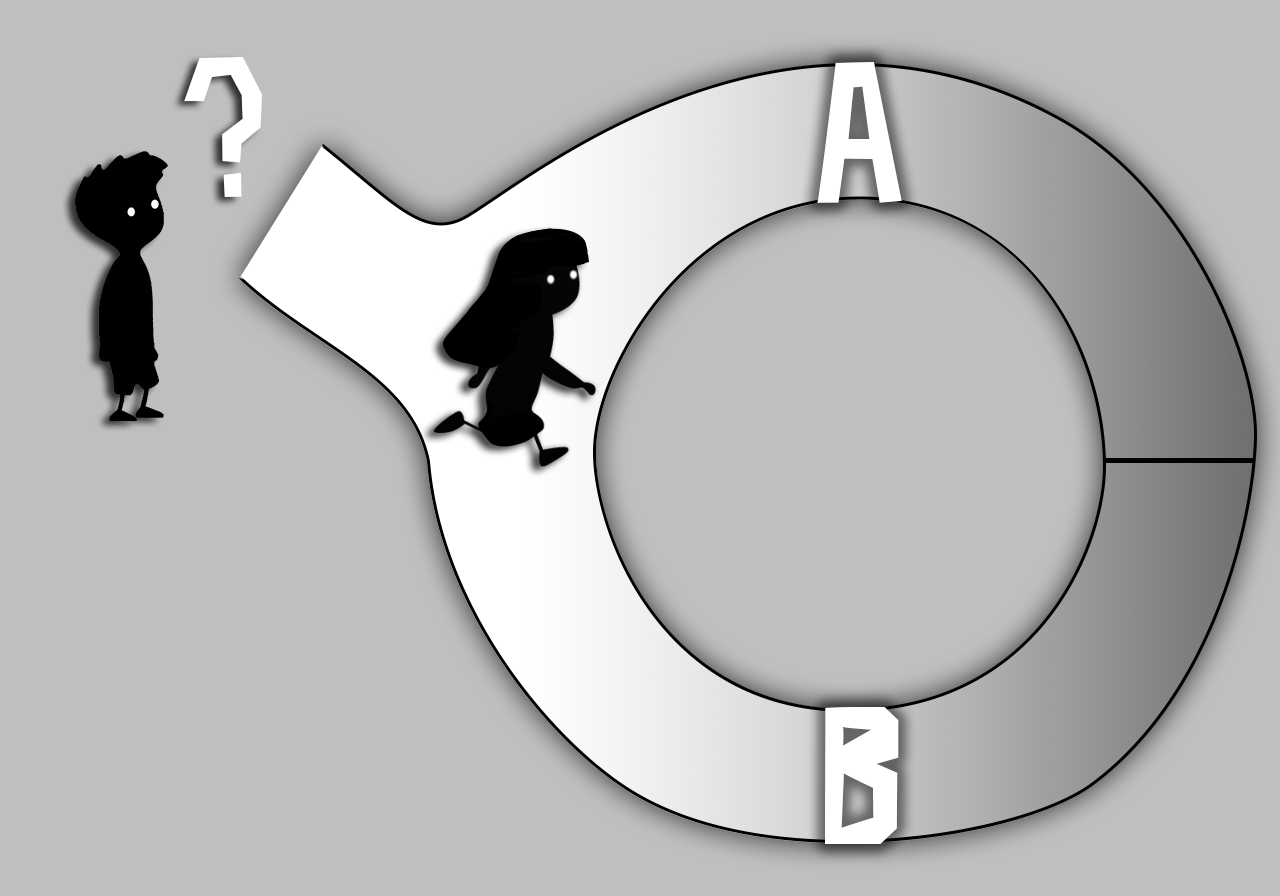
\includegraphics[width=1.\linewidth]{gfx/graficoJL_ZKP_1}\\La cueva \citep{ZKPcave:fig}
. Peggy entra por A o B al azar. Víctor espera fuera.}
Peggy y Víctor quedan en la entrada de la cueva con unos \textit{walkie-talkies}, de modo que Víctor esperará fuera y Peggy entrará a la cueva y tomará uno de los pasillos, que llamaremos A y B, sin decirle cuál a Víctor.

%\begin{figure}[bth]
%	\begin{center}
%		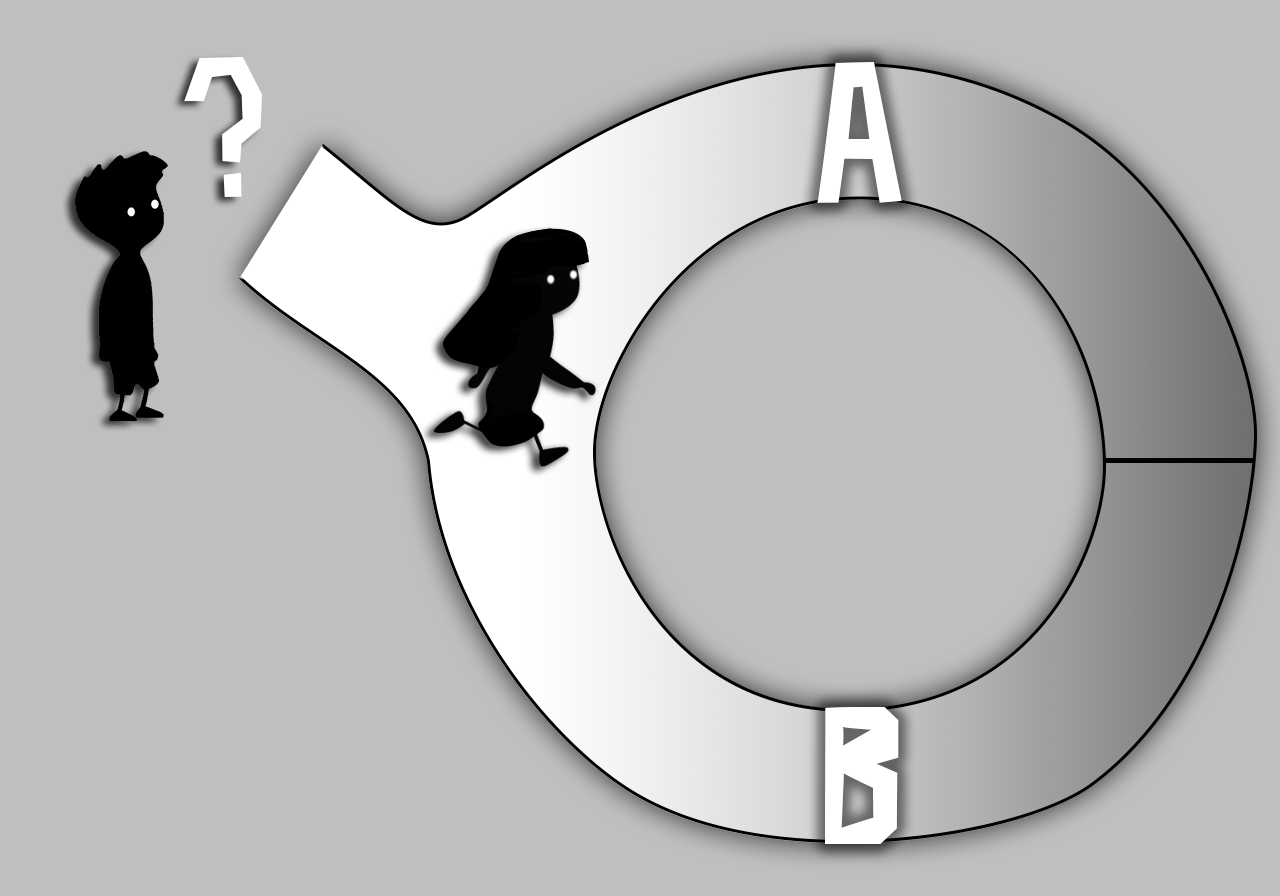
\includegraphics[width=.45\linewidth]{gfx/graficoJL_ZKP_1}
%	\end{center}
%	\caption{La cueva \citep{ZKPcave:fig}. Peggy entra por A o B al azar, Víctor espera fuera.}
%	\label{fig:ZKPcave1}
%\end{figure}

Al llegar a la puerta, avisa a Víctor para que entre a la cueva y espere en la bifurcación, donde \textbf{V}íctor, para intentar \textbf{v}erificar que Peggy conoce la clave, le indicará por qué pasillo quiere que vuelva, el A o el B.


%\begin{figure}[bth]
%	\begin{center}
%		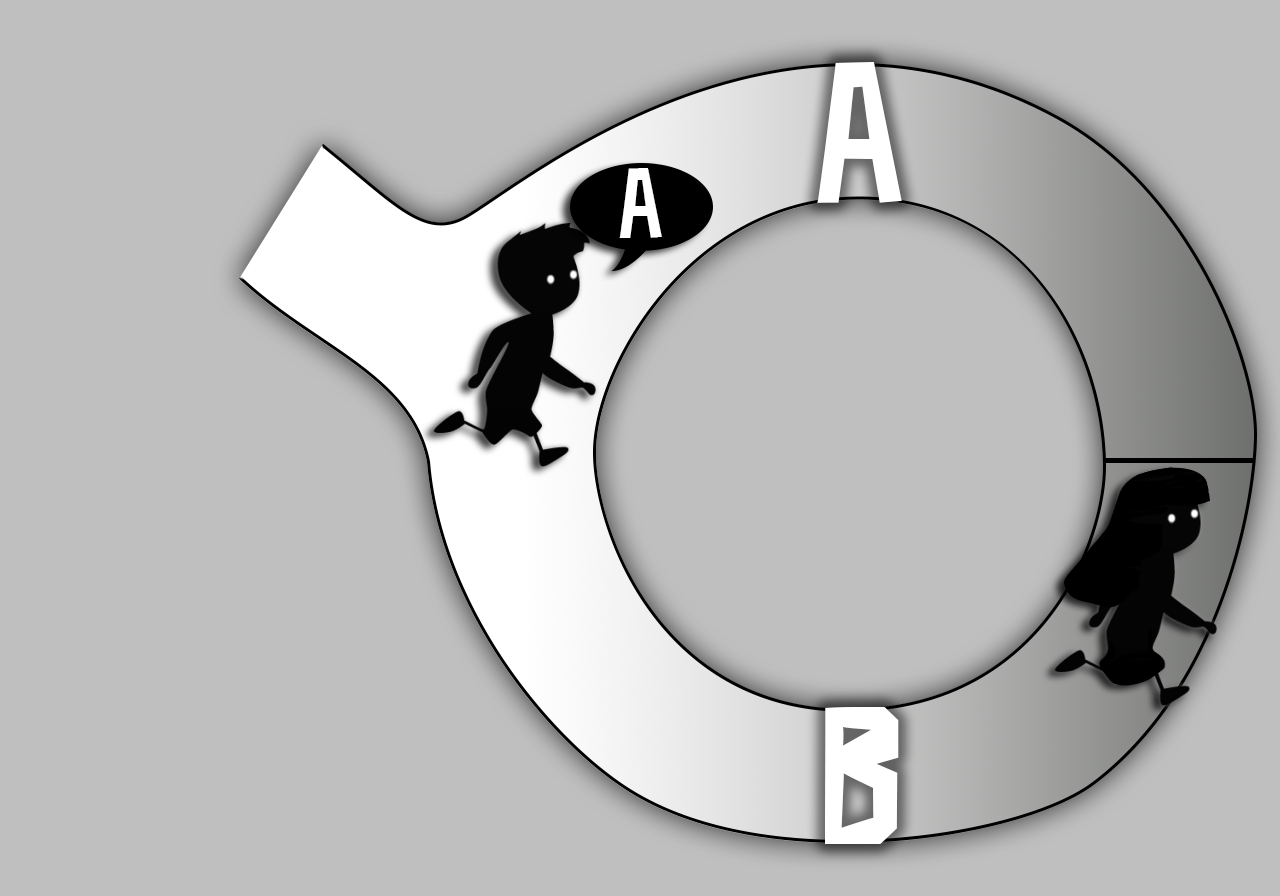
\includegraphics[width=.45\linewidth]{gfx/graficoJL_ZKP_2}
%	\end{center}
%	\caption{La cueva. Víctor elige al azar por dónde quiere que regrese Peggy.}
%	\label{fig:ZKPcave2}
%\end{figure}

Si Peggy realmente conoce la clave, podrá volver a la bifurcación por el pasillo solicitado, abriendo, si es preciso, la puerta.\marginpar{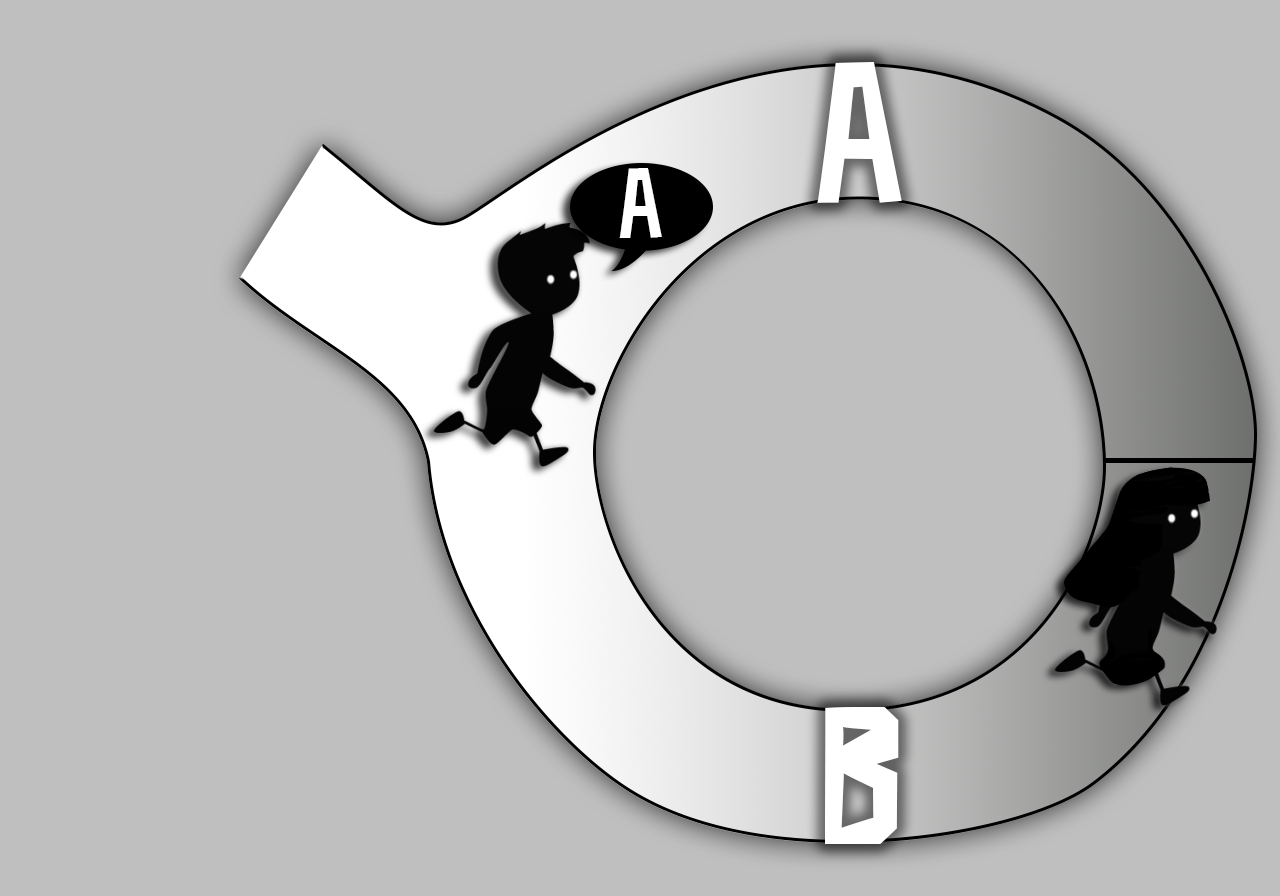
\includegraphics[width=1.\linewidth]{gfx/graficoJL_ZKP_2}\\La cueva. Víctor elige al azar por dónde quiere que regrese Peggy.}
En caso de que no conociera la clave, al entrar tenía una probabilidad del $50\%$ de adivinar qué pasillo pediría Víctor.


%\begin{figure}[bth]
%	\begin{center}
%		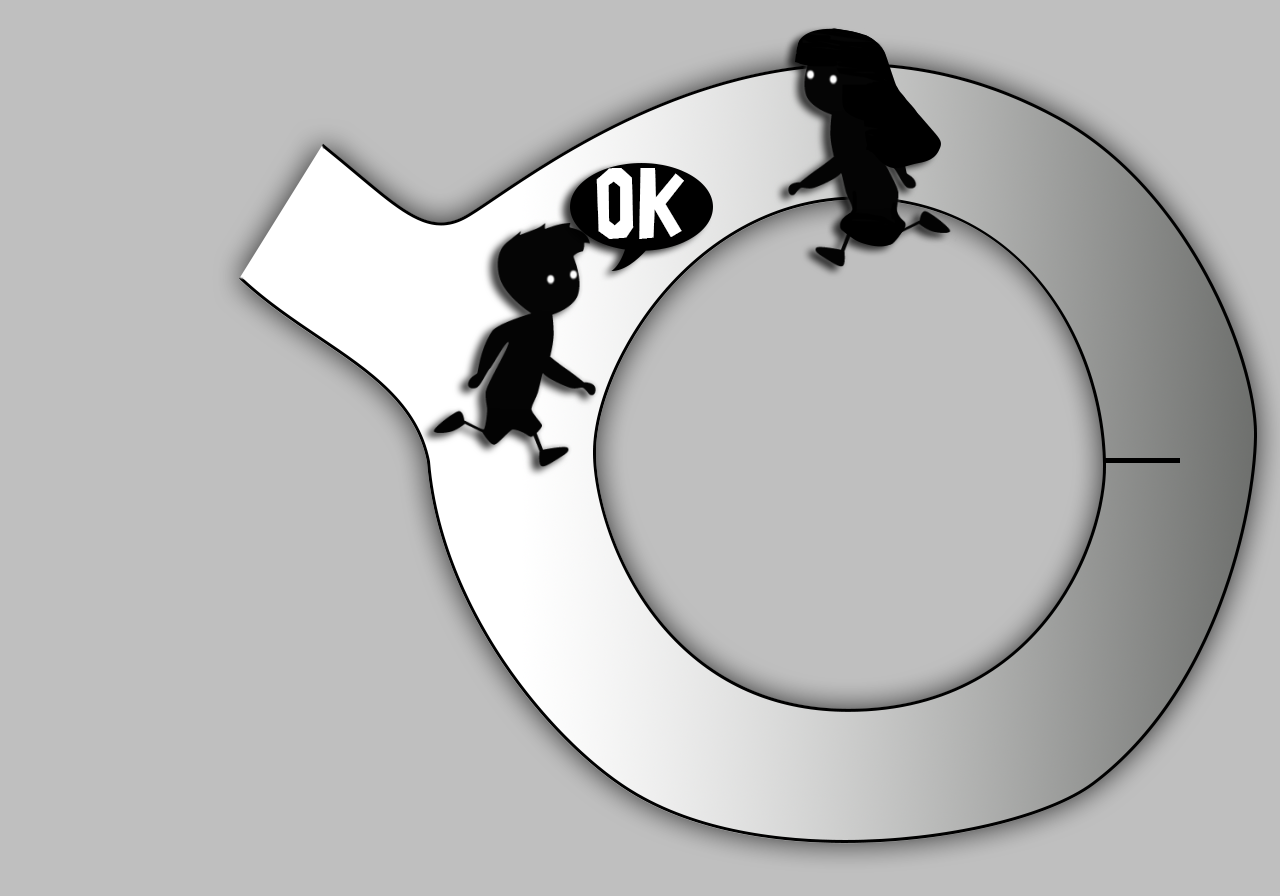
\includegraphics[width=.45\linewidth]{gfx/graficoJL_ZKP_3}
%	\end{center}
%	\caption{La cueva. Peggy vuelve por el camino pedido.}
%	\label{fig:ZKPcave3}
%\end{figure}

Víctor no se queda contento con una sola prueba, así que la repiten hasta que se convence. Si lo repitieran, por ejemplo, 20 veces, Peggy tendría solo una probabilidad de $2^{-20}$, prácticamente nula, de acertar todas las veces y engañar a Víctor.
\marginpar{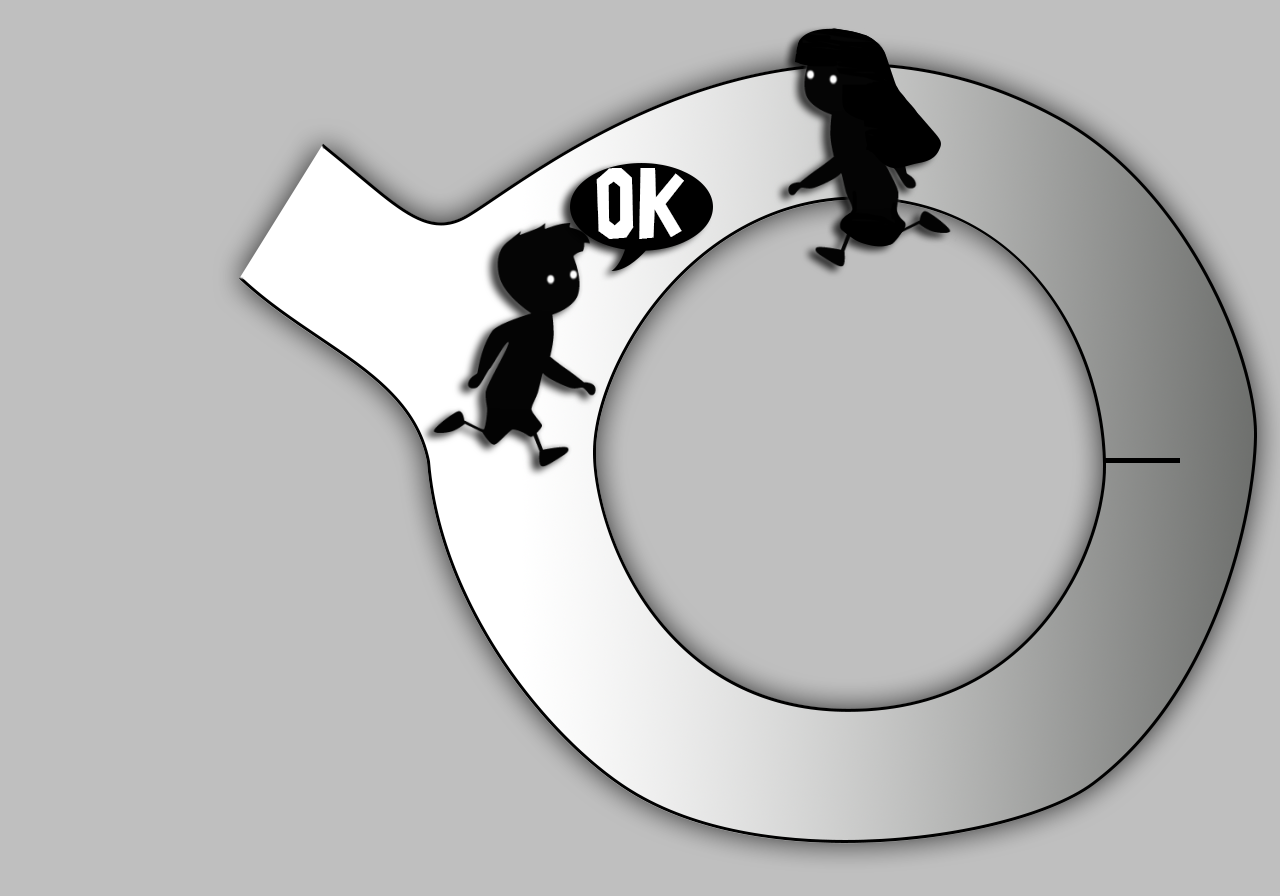
\includegraphics[width=1.\linewidth]{gfx/graficoJL_ZKP_3}\\La cueva. Peggy vuelve por el camino pedido.}


\textbf{E}va, curiosa de qué hacían Víctor y Peggy en la cueva, \textbf{e}spía a Víctor durante todo el proceso. Eva no sabe si Peggy y Víctor han acordado previamente qué pasillo pedir por el \textit{walkie-talkie}, y sólo Víctor está seguro de que los estaba eligiendo al azar.%, por eso, Eva no puede estar segura de si Peggy conoce la clave secreta, o bien estaban \textbf{s}imulando todo para engañarla por cotilla.

Más tarde Eva habla con Víctor, que está seguro de que Peggy conoce la clave, y éste querría convencer también a Eva, pero como él no conoce la clave, no puede repetir la prueba a Eva, sólo Peggy puede realizarla con éxito.
\end{quote}


\hfil

En el estudio formal de las Pruebas de Conocimiento Cero se utilizan distintos tipos de problemas en las áreas de \textbf{álgebra} y \textbf{grafos}, difíciles de resolver para quien no conoce algún secreto, equivalentes al problema de abrir la puerta sin conocer la clave. Los problemas más representativos de las Pruebas de Conocimiento Cero son el del logaritmo discreto, raíz cuadrada modular o residuos cuadráticos, y el isomorfismo de grafos.

Primero deberemos definir que un problema sea \textit{difícil}, y por ello en el capítulo TODO se presentarán unos preliminares de computación, que estudian y clasifican los problemas. A continuación, estudiaremos la teoría relacionada con cada uno de esos \textit{problemas difíciles}, en el capítulo TODO el álgebra relacionada con el logaritmo discreto, en el capítulo TODO las definiciones y teoremas necesarios sobre residuos cuadráticos, y en el capítulo TODO los conocimientos básicos de grafos necesarios para entender el problema.

Una vez conocemos las propiedades de cada uno, podremos estudiar en el capítulo TODO las Pruebas de Conocimiento Cero, definiendo qué propiedades deben cumplir y demostrando que cada una de las pruebas basadas en los anteriores problemas son de Conocimiento Cero. Finalmente, daremos algunas aplicaciones prácticas equivalentes a las de la criptografía actual.






















\hfil

BORRADOR:

Estructura:
\begin{itemize}
	\item Preliminares: Teoría ya dada en la carrera y que no necesita demostraciones
		\subitem Preliminares de computación: introducir problemas de decisión, clases de complejidad (para justificar qué problemas se usan en criptografía).
		\subitem Preliminares de álgebra: grupos y anillos, congruencias, id. de Bezout y alg. de Euclides extendido para los inversos. El problema del logaritmo discreto.
		\subitem Preliminares de grafos: definiciones básicas, coloración de grafos, problemas del isomorfismo de grafos y la 3-coloración.
		
	\item Residuos cuadráticos: indicar que es teoría de álgebra que no se da en la carrera y por eso dedicamos un capítulo a sus resultados.
		\subitem Definición, propiedades, símbolo de Legendre, símbolo de Jacobi, alg. raíces cuadradas, problema de residuosidad cuadrática.
		
	\item ZKP
		\subitem La historia de la cueva.
		\subitem Pruebas interactivas: completitud y robustez (soundness).
		\subitem ZKP: simulador.
			\subsubitem ZKP con residuos cuadráticos
			\subsubitem ZKP con isomorfismo de grafos
			\subsubitem ZKP con logaritmo discreto
		\subitem Otros tipos de ZKP: estadísticos, computacionales.
		
	\item Aplicaciones ZKP
		\subitem Firma utilizando un hash en vez de reto
		\subitem Protocolos de identificación
			\subsubitem Fiat-Shamir
			\subsubitem Feige-Fiat-Shamir
			\subsubitem Schnorr
			
			
	\item Implementaciones
\end{itemize}